% ============================================================================
% Draft manuscript, formatted for submission to a Royal Society journal
% (target: Royal Society Open Science, following the methodological precedent
% of Arcaute et al. 2016, R. Soc. Open Sci. 3:150691 -- see reference/papers/
% rsos.150691.pdf).
%
% This file uses the standard `article' class as a placeholder layout. The
% official RSOS LaTeX template (`rsos.cls'), available from the journal /
% Overleaf, is a drop-in replacement: swap the \documentclass line and the
% preamble below for the journal template's own preamble -- the section
% structure and content do not need to change.
% ============================================================================
\documentclass[11pt,a4paper]{article}

\usepackage[margin=1in]{geometry}
\usepackage{graphicx}
\usepackage{amsmath,amssymb}
\usepackage{booktabs}
\usepackage{authblk}
\usepackage[colorlinks=true,citecolor=blue,linkcolor=blue,urlcolor=blue]{hyperref}
\usepackage{natbib}
\usepackage{caption}
\usepackage{todonotes}

\title{Hierarchical percolation of travel time reveals spatial structure
  in the Roman road network}

\author[1]{Nishanth Kumar}
\affil[1]{[Affiliation -- to be completed]}

\date{}

\begin{document}

\maketitle

\begin{abstract}
We apply hierarchical agglomerative clustering (HAC) on travel-time
distances -- under single linkage, mathematically equivalent to a
percolation sweep over the network's own edges -- to the Roman road
network, with the aim of recovering spatial units of interest directly
from network connectivity rather than from imposed administrative
boundaries. Before turning to our own network, we calibrate the method
on the exact network and travel-time model used in a recent large-scale
reconstruction of the Roman road system, and show that it recovers that
network's Roman provinces with an Adjusted Rand Index (ARI) of 0.70
(bootstrap 95\% CI [0.68, 0.71]) at a threshold of $\sim$77 hours
($\sim$3.2 days) of travel -- confirming that the method can recover a
known administrative partition when one exists in the data. We then
apply the same percolation-equivalent clustering to our own,
independently constructed network of the Roman road system, where the
goal is not to reproduce this calibration result but to characterize
the emergent spatial units the network itself suggests. A first,
coarse benchmark against the Roman provinces on this network gives a
markedly weaker alignment (ARI $\approx 0.43$) with a less sharply
defined optimal threshold, which we read not as a replication failure
but as a signal that provincial administration is only one of several
candidate organizing principles the clustering may be picking up --
motivating a closer characterization of these units, and a comparison
against spatial/temporal null models, as the next step of this work.
\end{abstract}

\section{Introduction}
\todo[inline]{Introduction placeholder -- to be completed.}

\section{Methods}

\subsection{Data}

We work with two networks, referred to throughout by the names of the
directories holding their analysis in the accompanying repository:
\texttt{network1-single} (our own network; Section~\ref{sec:primary}) and
\texttt{network0-average} (the calibration network; Section~\ref{sec:validation}).
The name suffixes record the HAC linkage setting used for each (see
Section~\ref{sec:hac-method}) -- this is deliberate, since the two runs
are not directly comparable without accounting for it.

\paragraph{network1-single: the itinereX network (primary).}
Built from the raw Itiner-e linework \citep{desoto2025itinere}. Near-miss
junctions and duplicate endpoints are snapped, the linework is noded, and
degree-2 chains are simplified, giving a weighted graph of 8{,}460 nodes
and 12{,}849 edges across 12 connected components (see
\texttt{data\_cleaning/} in the accompanying repository). Edge weights
are travel times computed from edge length at a constant walking speed
of 2~km/h.

\paragraph{network0-average: the calibration network.}
To check that the method can recover a known administrative partition
before applying it to our own network, we separately run the same
general approach on the exact Itiner-e export and endpoint-noded
topology used by \citet{pazout2026network} (10{,}506 nodes, 14{,}770
edges, 13 connected components, including ferry links across the
Bosporus and the Dardanelles), with travel time computed from Tobler's
hiking function \citep{tobler1993hiking} applied to slope and geodesic
edge length. This self-contained calibration run is kept in
\texttt{results/HAC/network0-average/} and does not otherwise modify the
primary analysis.

\paragraph{Province boundaries.}
Both networks are overlaid with the Ancient World Mapping Center's
``Roman Empire AD 200'' province polygons, corrected by A.\ Pa\v{z}out
\citep{awmc2023provinces} (57 provinces). Each edge is assigned to the
province containing its midpoint, falling back to the province with the
longest geometric overlap when the midpoint falls outside every
polygon; nodes inherit the province of their incident within-province
edges. Edges that cross a provincial boundary, or that cannot be
assigned to any province, are excluded from the alignment scoring
described below.

\subsection{Hierarchical agglomerative clustering and percolation}
\label{sec:hac-method}

Following the general approach of \citet{arcaute2016cities}, who use a
percolation sweep over distance thresholds between street intersections
to recover the hierarchical regional and urban structure of Britain, we
apply an equivalent percolation sweep to travel time on the Roman road
network itself, rather than to Euclidean distance between unconnected
points.

Within each connected component, we compute pairwise travel-time
distances between nodes and perform hierarchical agglomerative
clustering (HAC; \texttt{scipy.cluster.hierarchy.linkage}). For
\texttt{network1-single} we use \emph{single} linkage: because single
linkage merges clusters at the weight of the minimum edge connecting
them, cutting the resulting dendrogram at a travel-time threshold $t$
reproduces exactly the connected components of the network with all
edges of weight greater than $t$ removed -- i.e.\ HAC under single
linkage is mathematically equivalent to a percolation sweep over the
network's own edges, computed once per component rather than
independently at every threshold. This equivalence is the reason we
adopt single linkage for the primary analysis: the resulting clusters
are, by construction, genuine percolation clusters of the road network,
not an artefact of a particular clustering criterion.

The calibration network, \texttt{network0-average}, instead uses
\emph{average} linkage, which clusters by mean pairwise travel time
between cluster members and does not share the exact percolation
equivalence described above. This difference predates the present
analysis and is retained here deliberately, flagged by the
\texttt{-average}/\texttt{-single} suffixes on each network's directory
name, so that ARI/NMI values reported for the two networks in
Section~\ref{sec:results} are never read as directly comparable without
that caveat in mind.

Sweeping $t$ across the full range of merge heights gives, at each
threshold: the number of clusters, and the size of the largest cluster
relative to the network (the percolation curve). We additionally fit a
power law to the percolation curve over its emergent region.

\paragraph{Alignment with provinces.}
At each threshold $t$, we compare the resulting cluster labels to the
province labels of the nodes with a known province assignment, using
the Adjusted Rand Index \citep[ARI;][]{hubert1985comparing} and
Normalized Mutual Information \citep[NMI;][]{danon2005comparing}. ARI
ranges from 0 (random partition) to 1 (perfect agreement, up to cluster
relabelling); NMI ranges from 0 to 1 and does not penalize a finer
partition as harshly as ARI. We search exhaustively over every distinct
merge height for the threshold that maximizes ARI against the
provinces, and estimate a 95\% confidence interval on that best ARI (and
on the threshold it occurs at) by bootstrap resampling nodes with
replacement and re-selecting, for each resample, the best-scoring
threshold among those closest to the full-data optimum.

\section{Results}
\label{sec:results}

\subsection{Calibration: recovering a known administrative partition
  (network0-average)}
\label{sec:validation}

Before asking what spatial units our own network suggests, we first
check that the method is capable of recovering a known partition at
all, on a network and travel-time model we did not build ourselves.
Figure~\ref{fig:network0} shows the percolation curve and
snapshot cluster maps for the calibration network of
\citet{pazout2026network}, with Tobler-function travel times and AWMC
provinces (10{,}430 of 10{,}506 nodes have a known province).

Table~\ref{tab:validation} reports ARI and NMI at six representative
travel-time snapshots. Alignment with the provinces rises from
essentially zero at 6--12 hours, peaks around 1--3 days, and falls off
again as clusters grow beyond provincial scale.

\begin{table}[h]
\centering
\caption{Province alignment at fixed travel-time snapshots, calibration
  network (network0-average; \citet{pazout2026network}, Tobler-function
  travel time; $n=10{,}430$ nodes with known province).}
\label{tab:validation}
\begin{tabular}{lrrr}
\toprule
Snapshot & Clusters & ARI & NMI \\
\midrule
6 h   & 2{,}809 & 0.039 & 0.640 \\
12 h  & 1{,}376 & 0.092 & 0.683 \\
24 h  & 514     & 0.201 & 0.734 \\
2 d   & 154     & 0.516 & 0.803 \\
7 d   & 22      & 0.493 & 0.778 \\
12 d  & 15      & 0.308 & 0.689 \\
\bottomrule
\end{tabular}
\end{table}

An exhaustive search over every merge height finds a single, sharp peak
at $t = 77.1$ hours ($\sim$3.2 days), with ARI $= 0.695$ (95\% bootstrap
CI $[0.681, 0.710]$). The peak is stable: every bootstrap resample of
the node set selects the same 77-hour merge height as optimal. At this
threshold the network's emergent regions correspond closely to the
Roman provincial map.

\begin{figure}[h]
\centering
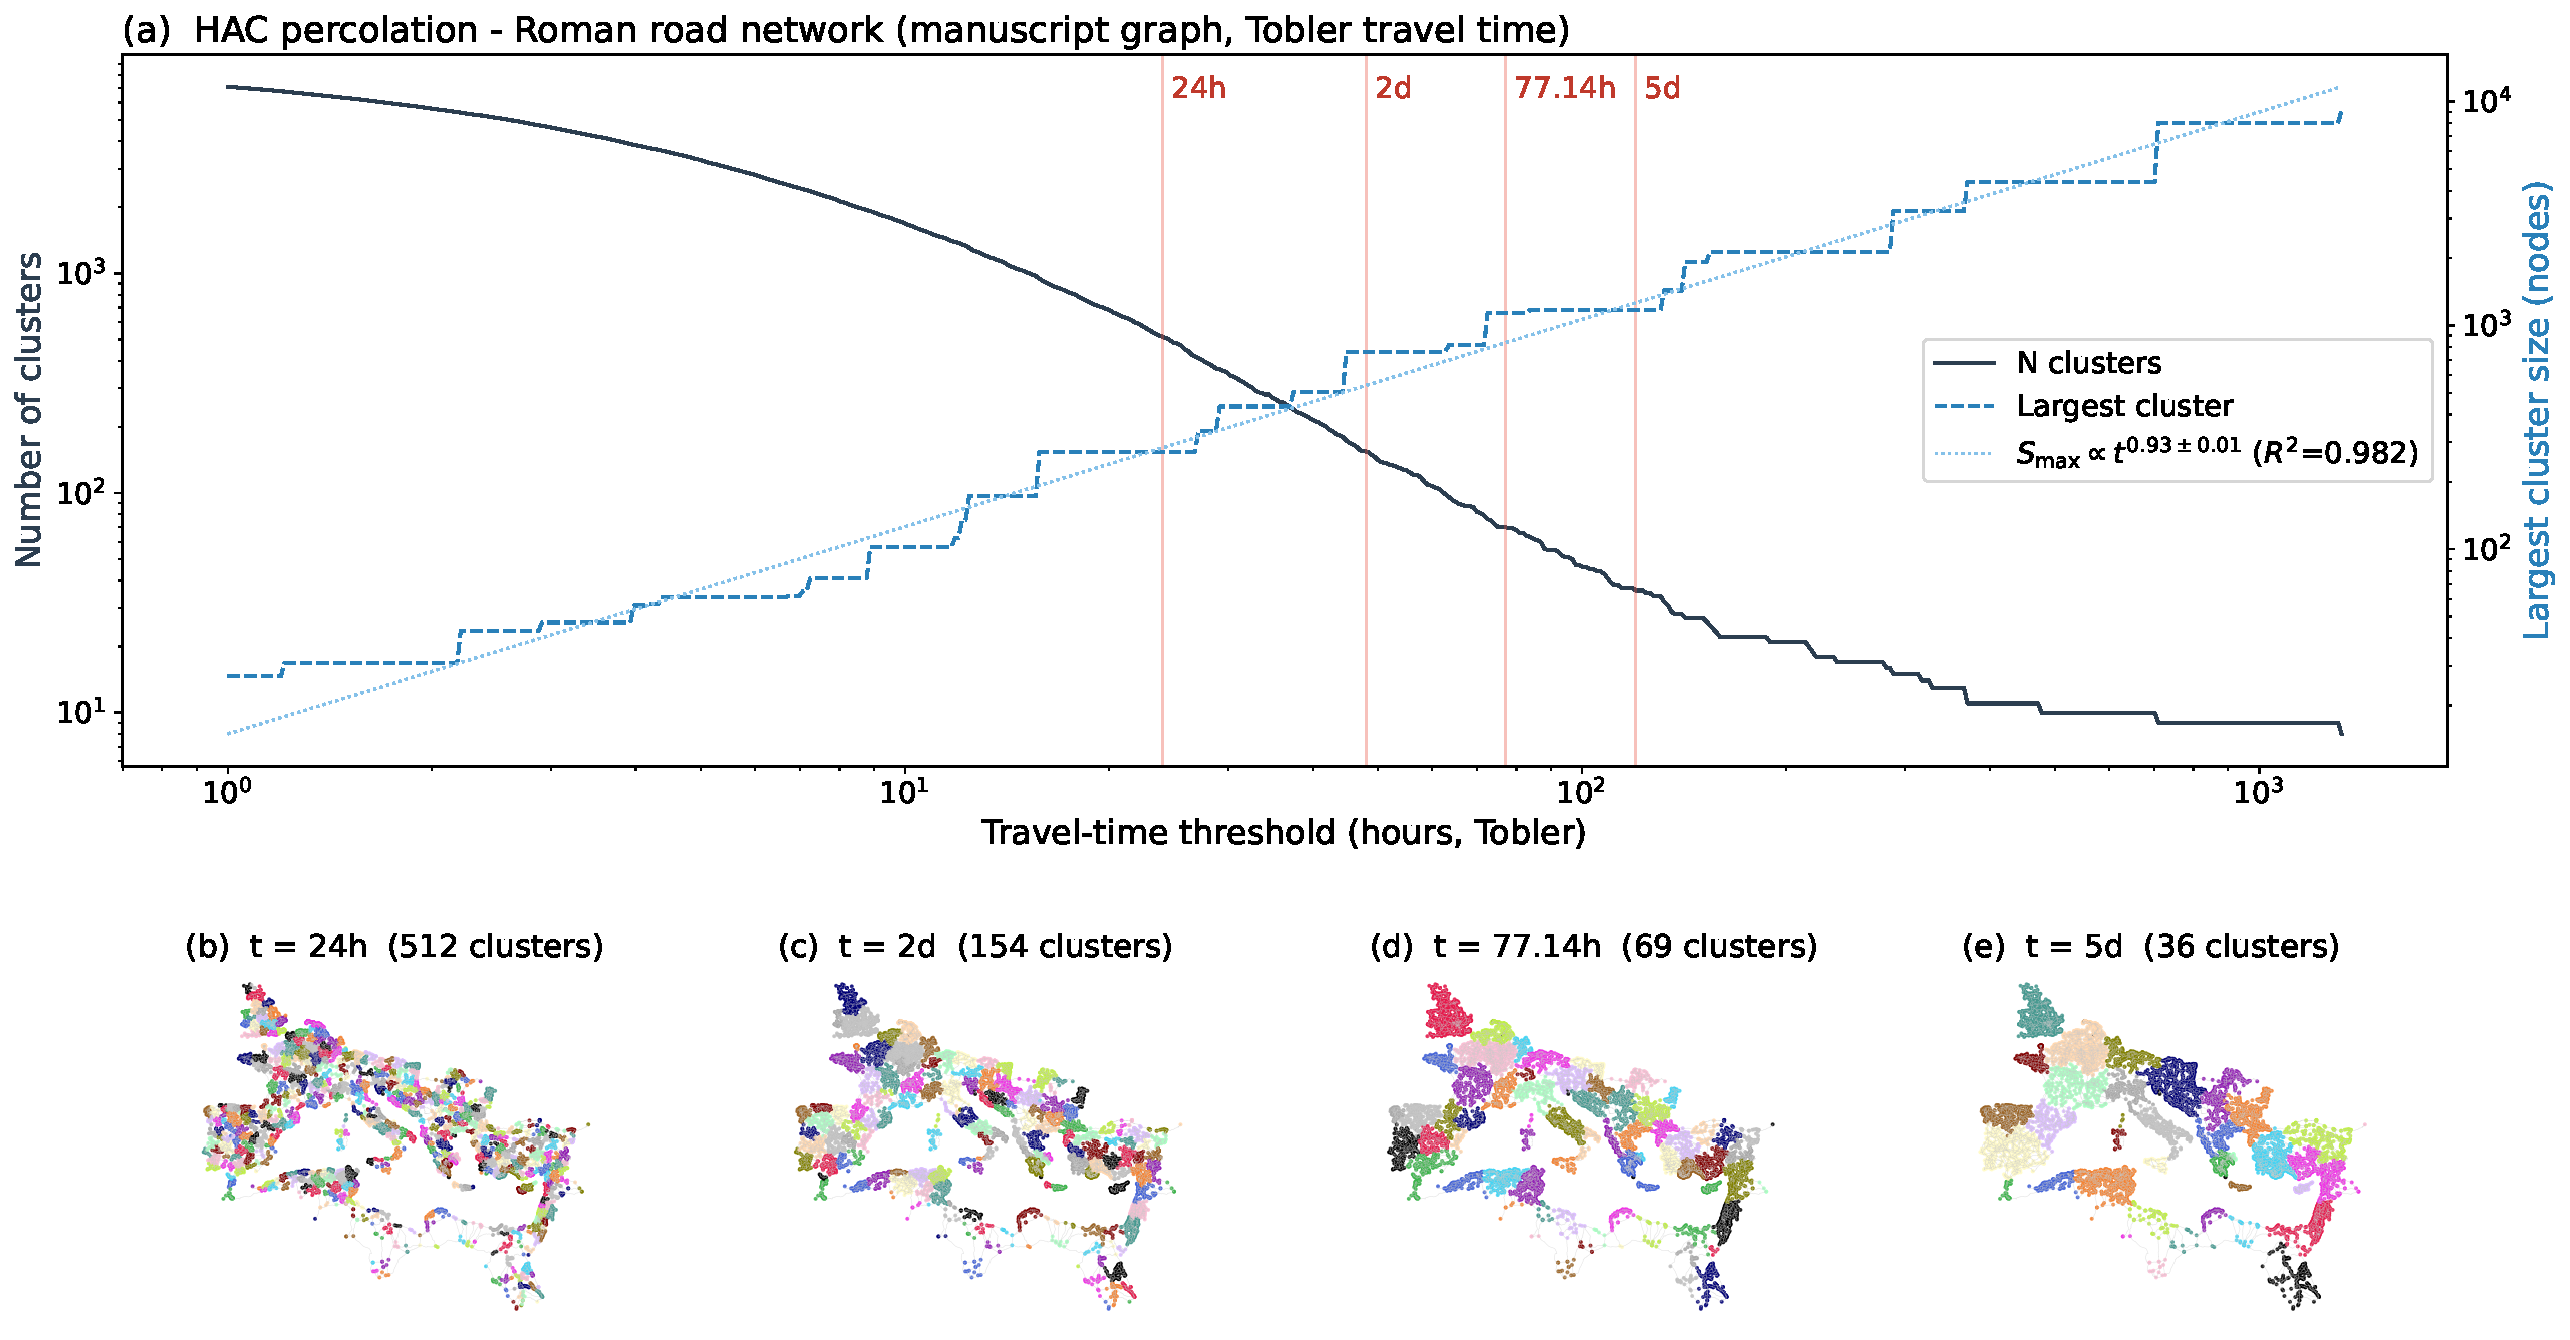
\includegraphics[width=\textwidth]{figures/fig1_network0-average_percolation.pdf}
\caption{Percolation curve and snapshot cluster maps for the calibration
  network (\texttt{results/HAC/network0-average/maps/hac\_percolation\_combined.pdf}).}
\label{fig:network0}
\end{figure}

\subsection{Towards emergent spatial units in the itinereX network
  (network1-single)}
\label{sec:primary}

Having confirmed in Section~\ref{sec:validation} that percolation-equivalent
HAC can recover a known administrative partition when one is present, we
turn to the question this paper is actually about: what spatial units does
the itinereX network itself suggest, under its own independently built
topology and a simple constant-speed (2~km/h) travel-time model? This is
not a replication of Section~\ref{sec:validation} -- we are not trying to
reproduce its ARI on a different network, and treating the comparison that
way would misread what each run is for. Section~\ref{sec:validation}
establishes that the method works; this section applies it, for the first
time, to a network nobody has clustered before, with the goal of
characterizing the clusters themselves as candidate spatial units, of
which provincial alignment is only one possible interpretation among
several worth testing.

As a first, coarse orientation, we benchmarked the resulting clusters
against the Roman provinces using the same ARI/NMI procedure as
Section~\ref{sec:validation}: an exhaustive search over every merge height
gives a best alignment of ARI $= 0.433$ (NMI $= 0.763$, 291 clusters) at
$t \approx 31.8$ hours, with a second, comparably good local optimum
around 25 hours rather than the single sharp peak seen in
Section~\ref{sec:validation} (95\% bootstrap CI on ARI $[0.426, 0.448]$;
on the threshold, $[24.8, 31.8]$ hours). We do not read this as a weaker
version of Section~\ref{sec:validation}'s result -- on a network built
under a different travel-time model, with its own topology, there is no
reason to expect the same number -- but as a preliminary signal that
provincial administration is detectable in, without fully explaining, the
clusters this network produces. We have deliberately not built a figure
or table around this number here: a single province-alignment statistic
does not do justice to what the clusters at each threshold actually look
like, and a closer, better-presented look at them is needed before drawing
conclusions from it.

\paragraph{What we take this to mean.}
The more interesting question this result raises is not ``why is the ARI
lower here'', but what the two comparable local optima, and the clusters
themselves, actually correspond to -- whether that is a different,
non-provincial regionalization of the network (e.g.\ against the Pleiades
regions already attached to this network's nodes), a boundary effect of
the constant-speed travel-time model, or a genuine feature of the
network's own topology. Distinguishing between these is the purpose of
comparing this run against the spatial/temporal null models in
\texttt{results/Null-models/}, which is ongoing work and not yet part of
this manuscript.

\section{Discussion}
\todo[inline]{Discussion placeholder -- to be completed. Note for later:
  the calibration run (Section~\ref{sec:validation}) establishes the
  method works; the open question for network1-single is what its
  emergent clusters represent, which needs (i) a proper figure/table once
  the clusters have had a closer look, and (ii) comparison against the
  null models in \texttt{results/Null-models/} to separate a genuine
  topological signal from an artefact of the constant-speed travel-time
  model.}

\section*{Data accessibility}
All code and data underlying this analysis are available in the
accompanying repository, under \texttt{results/HAC/network1-single/}
(primary analysis) and \texttt{results/HAC/network0-average/}
(calibration analysis).

\section*{Authors' contributions}
\todo[inline]{To be completed.}

\section*{Competing interests}
The authors declare no competing interests.

\section*{Funding}
\todo[inline]{To be completed.}

\bibliographystyle{unsrtnat}
\bibliography{refs}

\end{document}
